

\chapter{Finite State Machine}

\section{Introduction}


We seen in \autoref{chap:single_desing_flow} how to model sequential circuit using \verb|HLS| only. Now in this chapter we introduce a more formal approach known as \textit{state machine}.\\


An application can be modeled using state machine if we can:

\begin{itemize}

\item the task of application are the states

\item transition between states are determined using output in terms of inputs 


\end{itemize}

\todo{definition of state machine} \uti{definition of state machine}

\begin{itemize}

\item \textit{To re-write a more formal definition later when reviewing the theory of digital desing}

\end{itemize}


\subsection{FSM for a door lock}
\label{sub:fsm_door_lock}

Let's take an example shown in \autoref{fig:state_mch:lock_door_fsm}

\begin{figure}[h]
\centering
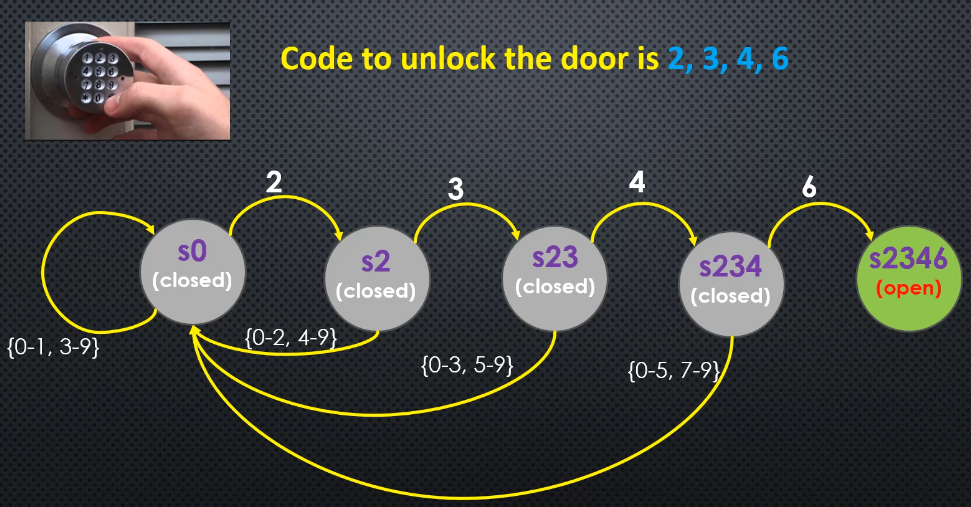
\includegraphics[scale=0.4,frame]{Figures/state_mch/lock_door_fsm}
\caption{State diagram for lock door example}
\label{fig:state_mch:lock_door_fsm}
\end{figure}

\begin{itemize}

\item The states are: either open or closed

\item The input are digits

\item We start the diagram by initial state $s_0$, where the door is initially closed.

	\begin{itemize}
	\item If it receives 2, we have transition to $s_2$
	
	\item If any digit besides 2, we don't have transition and we stay at $s_0$
	\end{itemize}

\item All the next states behaves with same concept

	\begin{itemize}
	\item If we have correct digit, transition to next state
	
	\item If not, no transition and we get back to $s_0$, since entering a wrong number force us to enter the whole sequence again from start
	\end{itemize}

\end{itemize}


\subsection{FSM for a digital signal}

An FSM can also be used to model some digital signal as shown in \autoref{fig:state_mch:fsm_digital_signal}.

\begin{figure}[h]
\centering
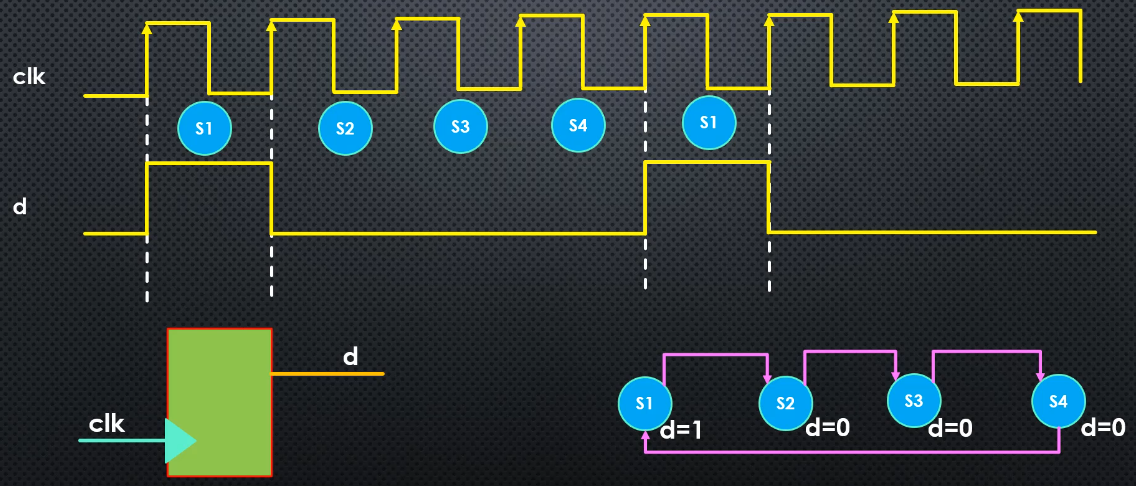
\includegraphics[scale=0.4,frame]{Figures/state_mch/fsm_digital_signal}
\caption{FSM to model a digital signal}
\label{fig:state_mch:fsm_digital_signal}
\end{figure}

\begin{itemize}
\item 1 period of $d$ require 4 clock cycles

\item Hence we can say that we have 4 states $s_n$

\item initial state $s_1$ is $d \,= \, 1$

\item All the 3 states have $d \, = \, 0$

\item \underline{Note:} the difference between this example and the example of \ref{sub:fsm_door_lock} it that we don't have conditions to move from 1 state to another

At each rising edge of the clock, we move from 1 state to another
\end{itemize}

\newpage
\subsection{Quiz}

\underline{Given:} draw the FSM for the signal diagram of \autoref{fig:state_mch:fsm_signal_quiz}.

\begin{figure}[h]
\centering
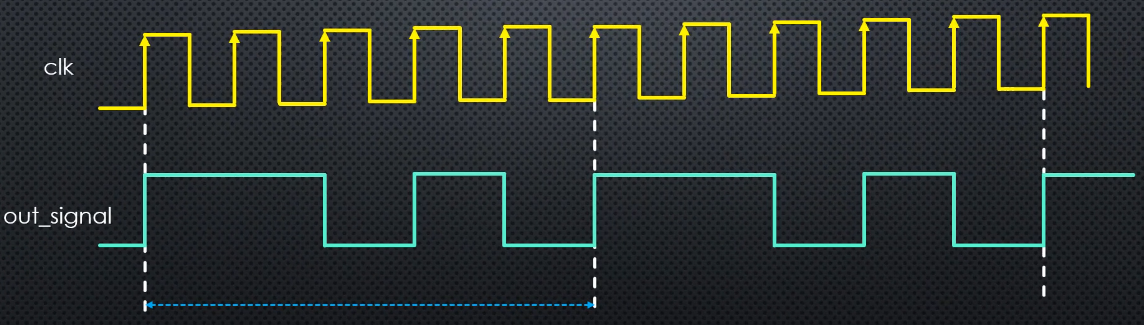
\includegraphics[scale=0.4,frame]{Figures/state_mch/fsm_signal_quiz}
\caption{FSM Quiz}
\label{fig:state_mch:fsm_signal_quiz}
\end{figure}

\underline{Solution:} shown in \autoref{fig:state_mch:fsm_signal_quiz_sol}. 

\begin{figure}[h]
\centering
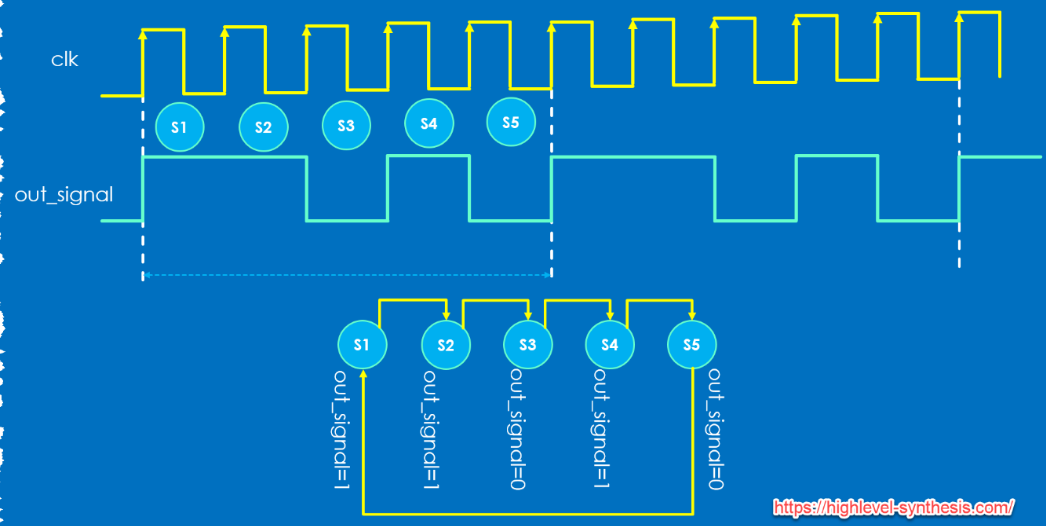
\includegraphics[scale=0.4,frame]{Figures/state_mch/fsm_signal_quiz_sol}
\caption{FSM Quiz}
\label{fig:state_mch:fsm_signal_quiz_sol}
\end{figure}





\newpage
\section{FSM Concept}
\label{sec:fsm_concept}

After seeing some examples, we explore the basic elements of FSM.

As mentioned before, FSM describe the behaviour of sequential circuits.\\

The 2 basic elements for an FSM are: states and transitions, as shown in \autoref{fig:state_mch:fsm_concept}.

\begin{figure}[h]
\centering
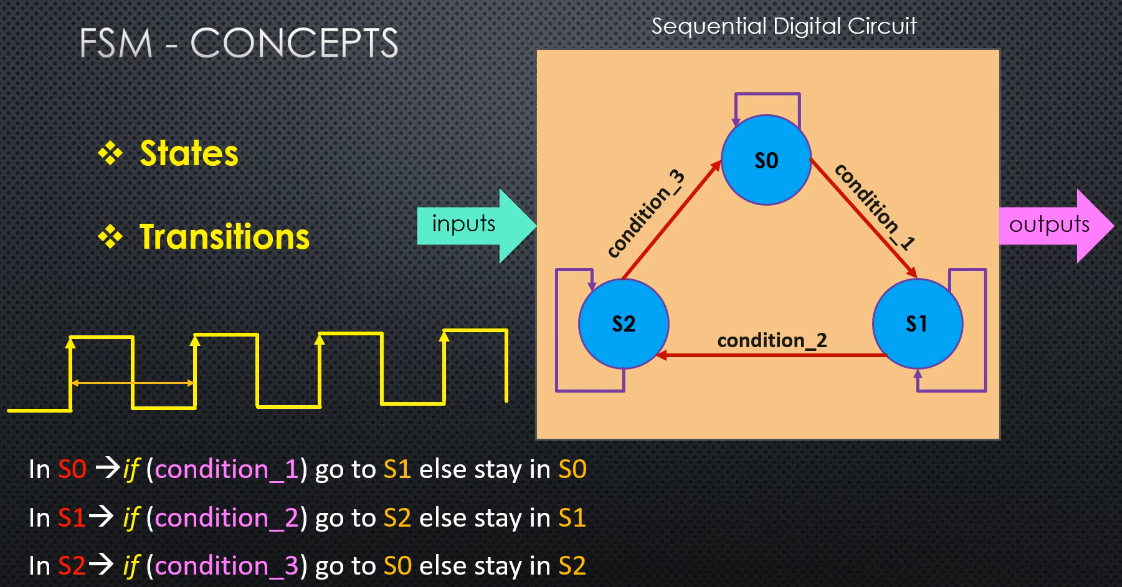
\includegraphics[scale=0.4,frame]{Figures/state_mch/fsm_concept}
\caption{FSM concept}
\label{fig:state_mch:fsm_concept}
\end{figure}

To implement these 2 elements, an FSM needs:

\begin{enumerate}

\item registers: to save the states

\item conditions to define transitions

\end{enumerate}


In this chapter we focus on:

\begin{itemize}

\item synchronous digial circuit: the clock is the same among all the components of the circuit

\item and we use single cycle approach

\end{itemize}

Since we are in single cycle approach, this means the transition between 2 states for an FSM occurs with a period of the clock.

Within this clock, if we met condition, we have a transition from $s_n \, \rightarrow \, s_{n \, + \, 1}$.

The conditions depends either on the states itself, or the ciruit input.


\newpage
\section{Code Template}

Now we move to \verb|HLS| code, where we give a general template we use when implementing FSM in \verb|HLS|. The template is shown in \autoref{fig:state_mch:fsm_template}.


\begin{figure}[h]
\centering
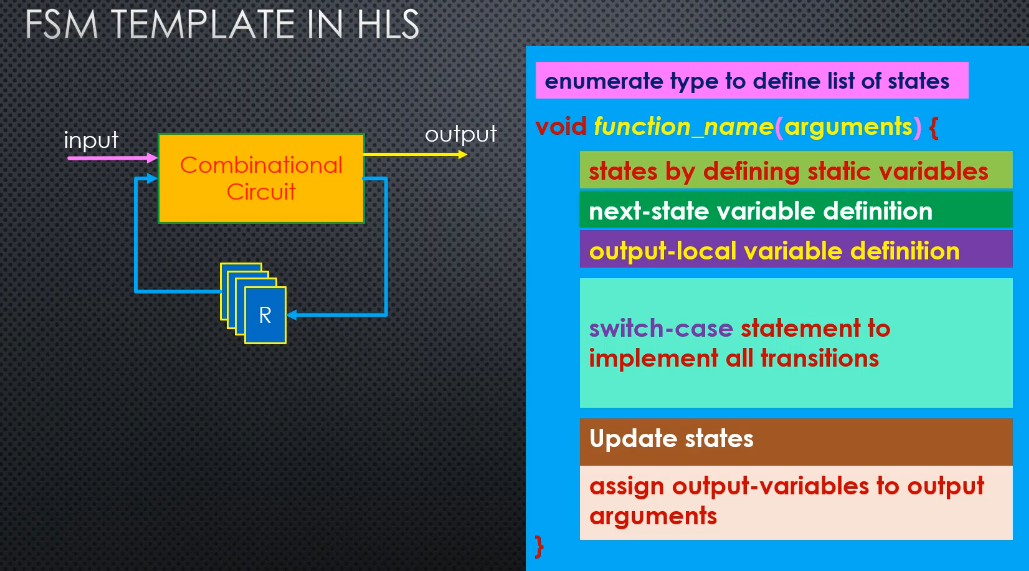
\includegraphics[scale=0.4,frame]{Figures/state_mch/fsm_template}
\caption{FSM code template}
\label{fig:state_mch:fsm_template}
\end{figure}

\begin{itemize}

\item states are defined by \verb|enum| data

\item Define some temporary variables in the body of the function, so we don't change our states register or output variable several times

	\begin{itemize}
	\item That's why we use \verb|next_state| variable to change it, and then at the end of the function we assign the final value to the original \verb|state| variable
	
	
	\item The reason behind this technique it may increase the design latency in newer versions of \verb|Vitis-HLS|.
	
	\end{itemize}

\end{itemize}

\newpage
\subsection{Door Lock HLS code}
To have a more concrete idea about template in practice, we take the door lock example seen in \ref{sub:fsm_door_lock}. Its FSM implemented in \verb|HLS| is shown in \autoref{fig:state_mch:fsm_template_door_lock}.

\begin{figure}[h]
\centering
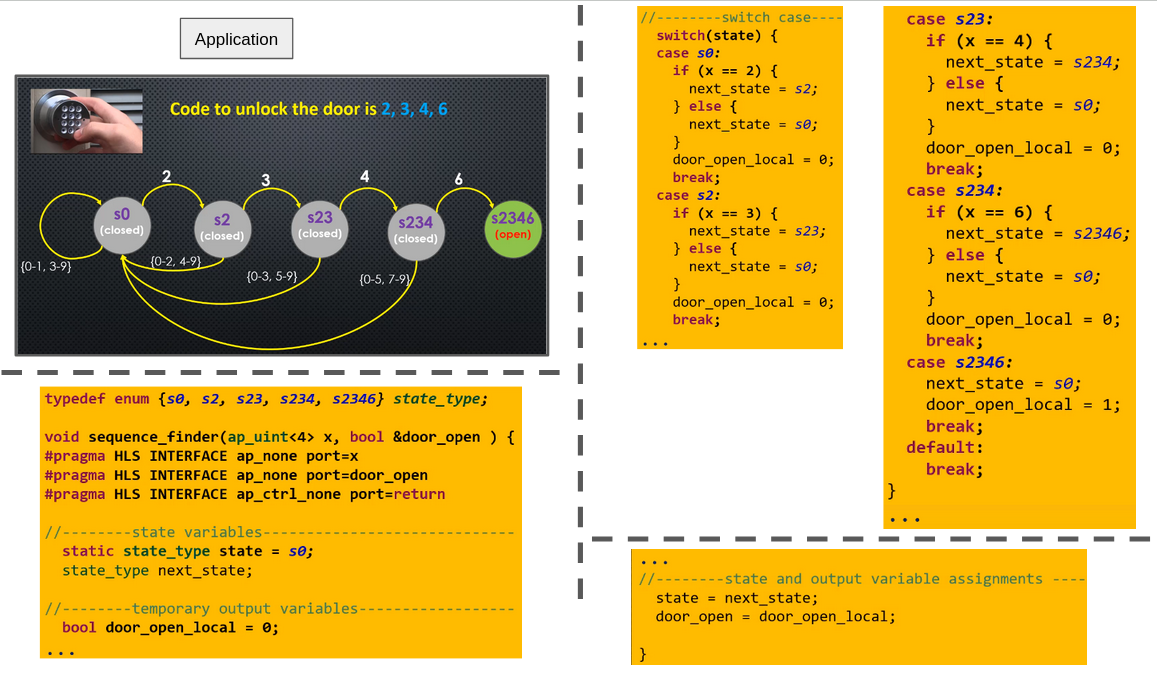
\includegraphics[scale=0.4,frame]{Figures/state_mch/fsm_template_door_lock}
\caption{FSM code template}
\label{fig:state_mch:fsm_template_door_lock}
\end{figure}


\newpage
\section{Summary State Machine}

\underline{Definition:}

\begin{itemize}

\item Finite state machine: technique describing sequential circuits

\end{itemize}


\underline{State machine concepts (\ref{sec:fsm_concept}) :}

\begin{itemize}

\item component of state machine (theory and modeling): states and transitions
	
\item Implementation:

	\begin{enumerate}
	\item registers to save states
	
	\item conditions to implement transition
	\end{enumerate}

\end{itemize}

	
\underline{Desing assumption taken into considerarion in this chapter (\ref{sec:fsm_concept}):}


\begin{itemize}

\item synchronous digial circuit:  same clock among all the components of the circuit

\item single cycle approach

	\begin{itemize}
	\item transition between 2 states for an
FSM occurs with a period of the clock

	\item Within this clock, if we met condition, we have a transition from $s_n \, \rightarrow \, s_{n \, + \, 1}$
	\end{itemize}


\end{itemize}
